
\documentclass{article}
\usepackage{natbib}
\usepackage[utf8]{inputenc}
\usepackage{geometry}
 \geometry{
 a4paper,
 total={170mm,257mm},
 left=20mm,
 top=20mm,
 }
 \usepackage{graphicx}
 \usepackage{subcaption}
 \usepackage{titling}
 \usepackage{float}
 \usepackage{amsmath}
\usepackage{listings}
\usepackage{color}
\usepackage{tikz}
\usepackage{graphicx}
\usepackage{caption}
\usepackage{subcaption}
\usepackage{tikz}
\usepackage{pgfplots}
\usetikzlibrary{spy,calc}
\usepackage{hyperref}

 \title{ASSIGNMENT 2: Computer Vision 792}
\author{Madhia Shabih}
\date{August 2024}
 
 \usepackage{fancyhdr}
\fancypagestyle{plain}{%  the preset of fancyhdr 
    \fancyhf{} % clear all header and footer fields
    \fancyfoot[L]{\thedate}
    \fancyhead[L]{24397644}
    \fancyhead[R]{\theauthor}
}
\makeatletter
\def\@maketitle{%
  \newpage
  \null
  \vskip 1em%
  \begin{center}%
  \let \footnote \thanks
    {\LARGE \@title \par}%
    \vskip 1em%
    %{\large \@date}%
  \end{center}%
  \par
  \vskip 1em}
\makeatother

\usepackage{lipsum}  
\usepackage{cmbright}

\title{Computer Vision Report: Camera Matrix and Epipolar Geometry}
\author{Your Name}
\date{\today}

\begin{document}
\maketitle

\section{Problem 1: Computing a Camera Matrix}

\subsection{1a: World Coordinate System and Camera Matrix Calculation}
\textbf{Description:} \\
% Explain how you chose the world coordinate axes and identified at least 28 corner points on the object in "lego1.jpg". 
% Describe the method used to determine the 2D image coordinates and 3D world coordinates. Include a table of correspondences if necessary.
Figure \ref{fig:lego1} below describes how I chose the world coordinate axes and Table 1 below includes the table of correspondences.  
\begin{figure}[H] % The [H] option places the figure exactly here
    \centering
    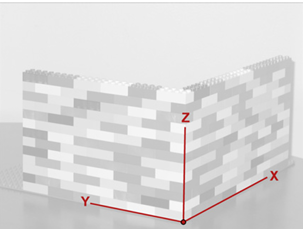
\includegraphics[width=0.3\textwidth]{axis.png} % Adjust the width as needed
    \caption{3D world co-ordinate system}
    \label{fig:lego1}
\end{figure}

\begin{table}[H]
    \centering
    \begin{tabular}{|c|c|c|c|c|c|}
    \hline
    \textbf{x} & \textbf{y} & \textbf{x'} & \textbf{y'} & \textbf{z'} \\
    \hline
    1547 & 1840 & 0   & 0   & 0     \\
    1557 & 1267 & 0   & 0   & 67.2  \\
    1562 & 937  & 0   & 0   & 105.6 \\
    1073 & 1749 & 0   & 64  & 0     \\
    404  & 1606 & 0   & 160 & 0     \\
    1873 & 1659 & 80  & 0   & 0     \\
    2328 & 1418 & 208 & 0   & 0     \\
    1430 & 1494 & 16  & 0   & 38.4  \\
    732  & 1372 & 0   & 112 & 38.4  \\
    961  & 1097 & 0   & 80  & 76.8  \\
    302  & 985  & 0   & 176 & 76.8  \\
    1320 & 901  & 0   & 32  & 105.6 \\
    849  & 827  & 0   & 96  & 105.6 \\
    409  & 771  & 0   & 160 & 105.6 \\
    1188 & 1611 & 0   & 48  & 19.2  \\
    737  & 1530 & 0   & 112 & 19.2  \\
    305  & 1443 & 0   & 176 & 19.2  \\
    1746 & 1661 & 48  & 0   & 0     \\
    1993 & 1536 & 112 & 0   & 0     \\
    2219 & 1419 & 176 & 0   & 0     \\
    2430 & 1302 & 240 & 0   & 0     \\
    1819 & 1233 & 64  & 0   & 57.6  \\
    2066 & 1129 & 128 & 0   & 57.6  \\
    2283 & 1020 & 192 & 0   & 57.6  \\
    2026 & 684  & 112 & 0   & 124.8 \\
    2357 & 561  & 208 & 0   & 124.8 \\
    852  & 745  & 0   & 96  & 124.8 \\
    198  & 653  & 0   & 192 & 124.8 \\
    \hline
    \end{tabular}
    \caption{2D Image Coordinates in Pixels and Corresponding 3D World Coordinates in mm}
    \end{table}

\textbf{Results:} \\
% Present the calculated camera matrix \(P\). Use the formula and explain briefly.
Below is the calculated P matrix: 

\[
P = \begin{bmatrix}
-6.26805785 \times 10^{12} & 2.24941247 \times 10^{8} & 4.52730087 \times 10^{-3} & 1.54665375 \times 10^{3} \\
-9.78591444 \times 10^{8}  & 3.66656339 \times 10^{8} & -8.62146328 & -1.83848493 \times 10^{3} \\
0 & 2.09637702 \times 10^{5} & -8.64770899 \times 10^{-5} & 1 
\end{bmatrix}
\]

\textbf{Discussion:} \\
Interpret the results, including any challenges encountered or assumptions made.

\subsection{1b: Proof of Camera Matrix Decomposition}
\textbf{Description:} \\
Outline the proof that the camera matrix decomposition algorithm returns \(K\), \(R\), and \(\tilde{C}\) such that \(K\) is upper-triangular, \(R\) is orthogonal, and \(KR[I - \tilde{C}]\) equals \(P\).

\textbf{Discussion:} \\
Comment on the extent of uniqueness in the decomposition and its importance.

\subsection{1c: Camera Matrix Decomposition for lego1.jpg}
\textbf{Results:} \\
% Show the decomposition of matrix \(P\) into \(K\), \(R\), and \(\tilde{C}\). Scale \(K\) such that its bottom-right entry is 1. Include the necessary calculations and matrices.
\subsection*{Intrinsic Matrix \(K\)}
\[
K = 
\begin{bmatrix}
2.58795903 \times 10^{-1} & 2.98994779 \times 10^{7} & 1.07299996 \times 10^{3} \\
0 & 4.66801265 \times 10^{3} & 1.74899999 \times 10^{3} \\
0 & 0 & 1
\end{bmatrix}
\]

\subsection*{Rotation Matrix \(R\)}
\[
R = \begin{bmatrix}
-8.65551697 \times 10^{-9} & 4.12507336 \times 10^{-10} & 1 \\
-1 & 2.22044605 \times 10^{-16} & -8.65551697 \times 10^{-9} \\
0 & 1 & -4.12507336 \times 10^{-10}
\end{bmatrix}
\]

\subsection*{Camera Center \(C\)}
\[
C = \begin{bmatrix}
6.89902951 \times 10^{-11} \\
-4.94485147 \times 10^{-6} \\
-4.23549166 \times 10^{2}
\end{bmatrix}
\]

\textbf{Discussion:} \\
Discuss the significance of the decomposed components.

\section{Problem 2: Computing a Second Camera Matrix}

\subsection{2a: Repeating the Calculations for lego2.jpg}
\textbf{Description:} \\

\begin{table}[h!]
    \centering
    \begin{tabular}{|c|c|c|c|c|}
    \hline
    \textbf{x} & \textbf{y} & \textbf{x} (3D) & \textbf{y} (3D) & \textbf{z} (3D) \\
    \hline
    240 & 1440 & 0 & 192 & 0 \\
    242 & 1308 & 0 & 192 & 19.2 \\
    240 & 1178 & 0 & 192 & 38.4 \\
    242 & 1045 & 0 & 192 & 57.6 \\
    245 & 905 & 0 & 192 & 76.8 \\
    245 & 786 & 0 & 192 & 96 \\
    250 & 577 & 0 & 192 & 124.8 \\
    988 & 1758 & 0 & 0 & 0 \\
    991 & 1623 & 0 & 0 & 19.2 \\
    988 & 1471 & 0 & 0 & 38.4 \\
    991 & 1320 & 0 & 0 & 57.6 \\
    993 & 1180 & 0 & 0 & 76.8 \\
    998 & 1028 & 0 & 0 & 96 \\
    998 & 799 & 0 & 0 & 124.8 \\
    2424 & 1506 & 240 & 0 & 0 \\
    2421 & 1366 & 240 & 0 & 19.2 \\
    2424 & 1236 & 240 & 0 & 38.4 \\
    2434 & 1109 & 240 & 0 & 57.6 \\
    2439 & 972 & 240 & 0 & 76.8 \\
    2439 & 837 & 240 & 0 & 96 \\
    2447 & 625 & 240 & 0 & 124.8 \\
    \hline
    \end{tabular}
    \caption{2D coordinates and their corresponding 3D coordinates}
    \end{table}

\subsubsection*{Homography Matrix}

The homography matrix \( P \) is given by:
\[
P = \begin{bmatrix}
-3.73942007 \times 10^{-3} & 6.00696271 \times 10^{-4} & 2.09880695 \times 10^{-15} & -1.15333684 \times 10^{-1} \\
-7.14513566 \times 10^{-3} & 6.10214747 \times 10^{-4} & 8.90213106 \times 10^{-14} & 1.17161231 \times 10^{-1} \\
0 & -5.20833333 \times 10^{-3} & 8.68057066 \times 10^{-18} & 1
\end{bmatrix}
\]

\subsubsection*{Intrinsic Matrix}

The intrinsic matrix \( K \) is given by:
\[
K = \begin{bmatrix}
8.54211707 \times 10^{-12} & 7.17968654 \times 10^{-1} & -1.15333684 \times 10^{-1} \\
0 & 1.37186605 & -1.17161231 \times 10^{-1} \\
0 & 0 & 1
\end{bmatrix}
\]

\subsubsection*{Rotation Matrix}

The rotation matrix \( R \) is given by:
\[
R = \begin{bmatrix}
-1.24591515 \times 10^{-11} & -1.66666957 \times 10^{-15} & -1.00000000 \\
-1.00000000 & 0 & 1.24591515 \times 10^{-11} \\
0 & -1.00000000 & 1.66666957 \times 10^{-15}
\end{bmatrix}
\]

\subsubsection*{Camera Center}

The camera center \( C \) is given by:
\[
C = \begin{bmatrix}
-1.54781397 \\
1.91995406 \times 10^2 \\
-2.75640741 \times 10^{12}
\end{bmatrix}
\]

\textbf{Results:} \\
Present the new camera matrix and the distance between the two camera centers and the angle between their principal axes.

\textbf{Discussion:} \\
Analyze the differences between the two matrices and what they imply about the relative camera positions.

\subsection{2b: 3D Plot of Camera Positions and World Points}
\textbf{Results:} \\
Include the 3D plot with labeled axes and camera positions. Provide different views to show the camera orientations.

\textbf{Discussion:} \\
Discuss how the plot clarifies the relative positions and orientations of the cameras.

\section{Problem 3: The Image of the World Coordinate System}
\textbf{Description:} \\
Prove that \(p_4\) is a homogeneous representation of the image of the world origin, and \(p_1, p_2, p_3\) are the images of the vanishing points of the world X, Y, and Z axes. Include mathematical derivations.

\textbf{Results:} \\
Demonstrate these statements using the two computed camera matrices. Include the plots of projected world axes overlaid on the images.

\textbf{Discussion:} \\
Interpret the results and any observations.

\section{Problem 4: Epipolar Geometry}

\subsection{4a: Calculating Epipoles}
\textbf{Description:} \\
Describe the method used to calculate the epipoles \(e\) and \(e'\).

\textbf{Results:} \\
Provide the de-homogenized coordinates of both epipoles and discuss whether the coordinates make sense.

\subsection{4b: Computing the Fundamental Matrix and Epipolar Lines}
\textbf{Description:} \\
Explain how the fundamental matrix \(F\) was computed from \(P\) and \(P'\).

\textbf{Results:} \\
Display the epipolar lines on both images. Describe the visualization approach, including the use of color for corresponding lines.

\textbf{Discussion:} \\
Analyze the correctness of the epipolar lines and any observations on the correspondence between features.

\section{Conclusion}
Summarize the key findings of the report, including the results of the camera matrix calculations, decomposition, and epipolar geometry analysis.

\section{References}
List any references, textbooks, or online resources you used.

\end{document}
